\documentclass[border=10pt]{standalone}

\usepackage{tikz}
\usepackage{tikzsymbols}
\usetikzlibrary{calc,patterns,shapes.geometric}

\def\centerarc[#1](#2)(#3:#4:#5){\draw[#1] ($(#2)+({#5*cos(#3)},{#5*sin(#3)})$) arc (#3:#4:#5);}

\begin{document}
	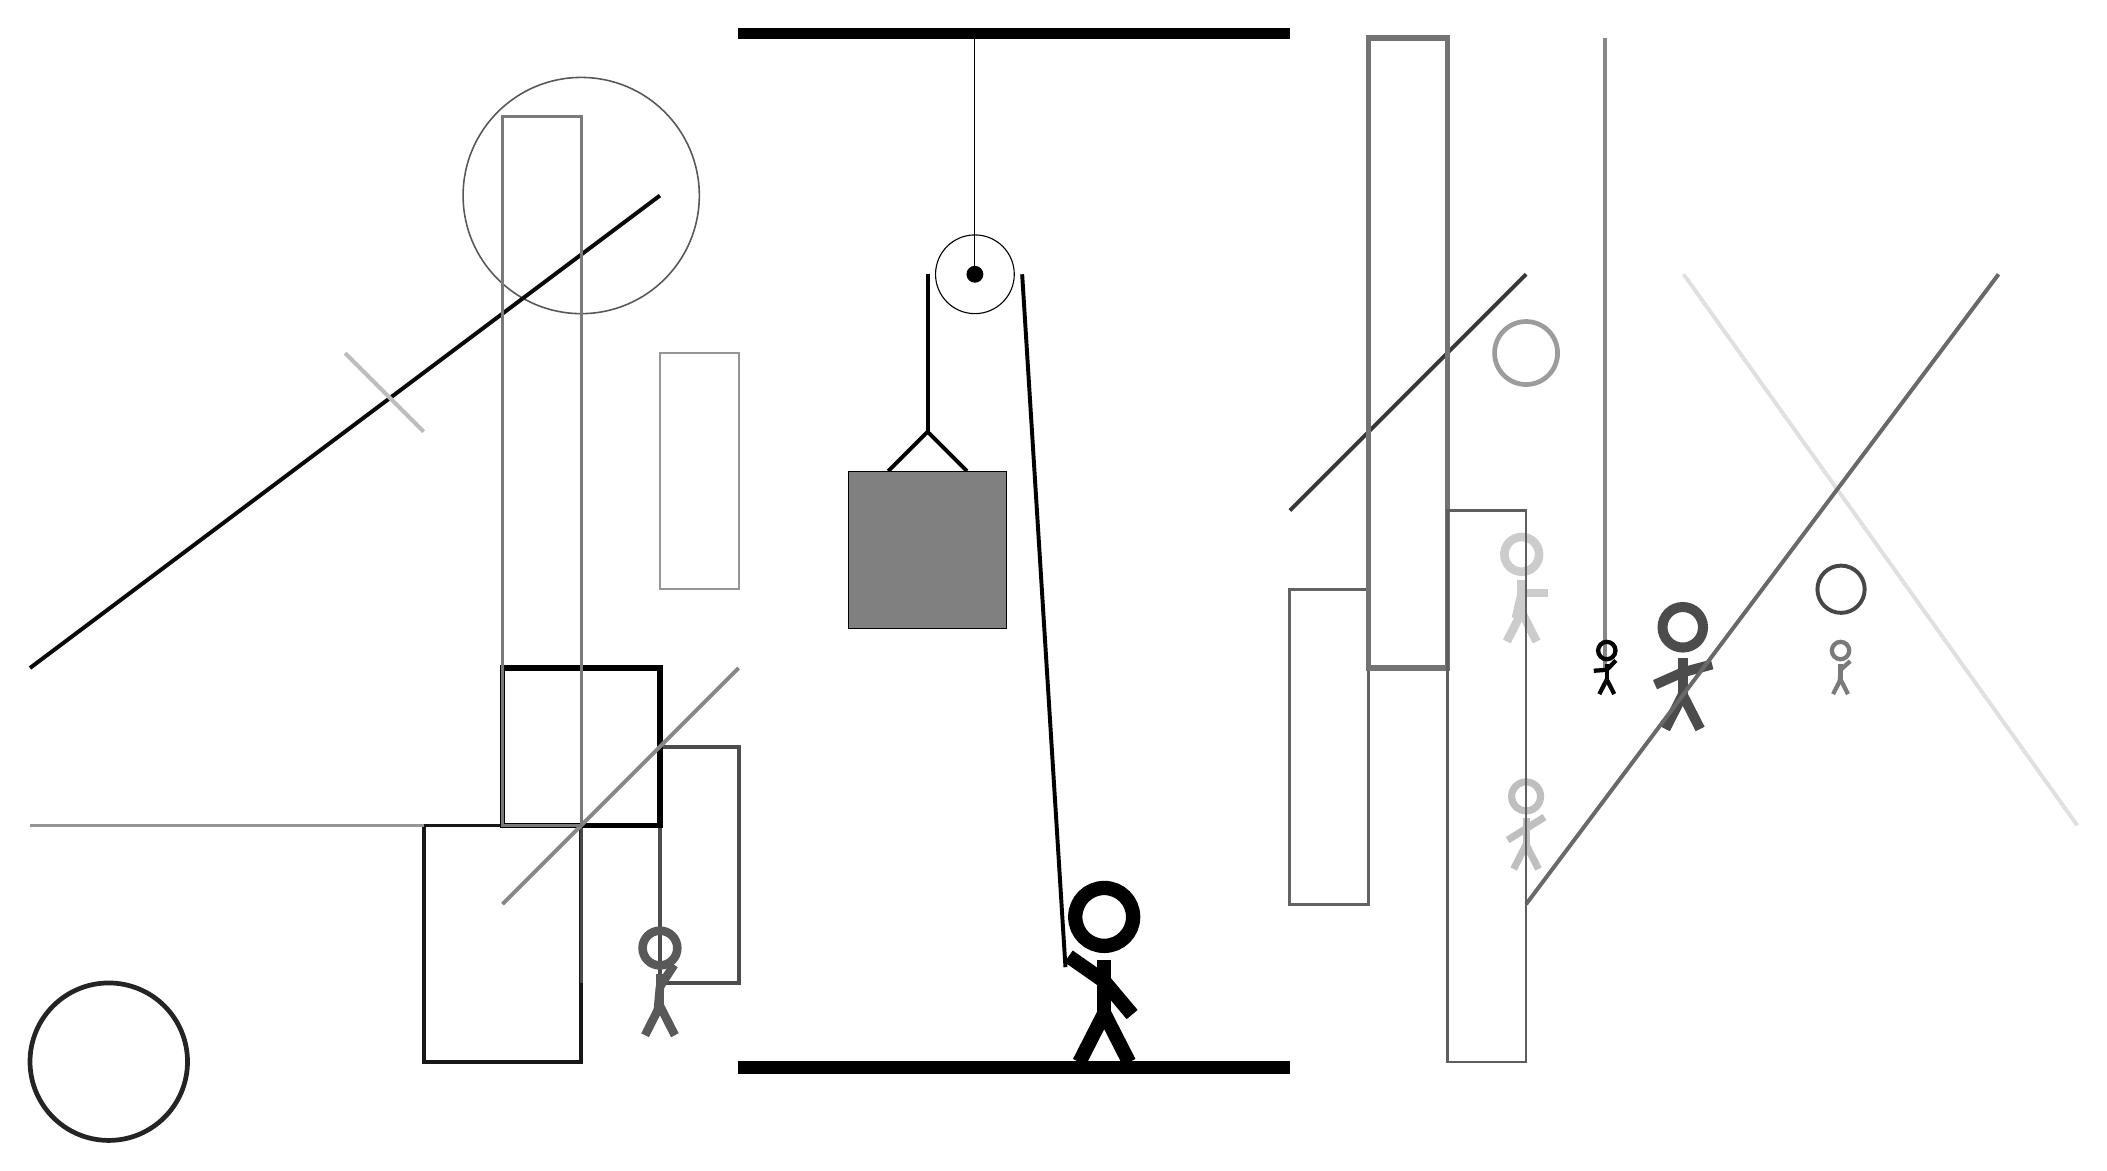
\begin{tikzpicture}
		%%%%% START %%%%%
		
		\draw[fill=black] (-2, 10) rectangle (5, 10.125);
		
		\draw (1, 7) circle (0.5);
		\draw[fill=black] (1, 7) circle (0.1);
		\draw (1, 10) -- (1, 7);
		
		\draw[line width=0.5mm] (-0.1, 4.5) -- (0.4, 5.0) -- (0.9, 4.5);
		\draw[fill=black!50] (-0.6, 4.5) rectangle (1.4, 2.5);
		
		\draw[line width=0.5mm] (0.4, 7) -- (0.4, 5.0);
		\centerarc[line width=0.5mm](1, 7)(0:180:0.6);
		\draw[line width=0.5mm](1.6, 7) -- (2.15, -1.8);
		
		\draw[line width=0.5mm, color=black!78](5, 4) -- (8, 7);
		
		\draw[line width=0.3mm, color=black!41] (-2, 6) rectangle (-3, 3);
		\draw [line width=0.2mm, color=black!66](-4, 8) circle (1.5);
		\draw[line width=0.5mm, color=black!91] (-4, 0) rectangle (-6, -3);
		\draw [line width=0.6mm, color=black!39](8, 6) circle (0.4);
		\node[line width=0.2mm, color=black!25] at (8, 0) {\Strichmaxerl[5][32][32]};
		\draw[line width=0.5mm, color=black!96](-3, 8) -- (-11, 2);
		
		\node[line width=0.4mm, color=black!70] at (10, 2) {\Strichmaxerl[7][24][15]};
		\draw[line width=0.5mm, color=black!47](9, 10) -- (9, 2);
		\node[line width=0.5mm, color=black!20] at (8, 3) {\Strichmaxerl[6][77][0]};
		
		\draw[line width=0.5mm, color=black!12](10, 7) -- (15, 0);
		\node[line width=0.3mm, color=black!52] at (12, 2) {\Strichmaxerl[3][86][42]};
		\node[line width=0.2mm, color=black!98] at (9, 2) {\Strichmaxerl[3][4][46]};
		
		\draw[line width=0.5mm, color=black!59](8, -1) -- (14, 7);
		\draw[line width=0.5mm, color=black!70] (-3, 1) rectangle (-2, -2);
		\draw[line width=0.4mm, color=black!61] (5, 3) rectangle (6, -1);
		\draw[line width=0.4mm, color=black!72] (-4, 4) rectangle (-4, -2);
		\draw [line width=0.6mm, color=black!86](-10, -3) circle (1.0);
		\draw [line width=0.5mm, color=black!72](12, 3) circle (0.3);
		\draw[line width=0.5mm, color=black!41](-6, 0) -- (-11, 0);
		\draw[line width=0.7mm, color=black!55] (6, 10) rectangle (7, 2);
		
		\node[line width=0.6mm, color=black!65] at (-3, -2) {\Strichmaxerl[6][85][57]};
		
		\draw[line width=0.7mm, color=black!100] (-3, 0) rectangle (-5, 2);
		\draw[line width=0.5mm, color=black!26](-7, 6) -- (-6, 5);
		\draw[line width=0.5mm, color=black!47](-2, 2) -- (-5, -1);
		
		\draw[line width=0.3mm, color=black!63] (7, 4) rectangle (8, -3);
		\draw[line width=0.4mm, color=black!52] (-4, 9) rectangle (-5, 0);
		
		\node at (2.6, -1.9) {\Strichmaxerl[10][-35][-50]};
		
		\draw[fill=black] (-2, -3) rectangle (5, -3.15);
		
		%%%%% END %%%%%
	\end{tikzpicture}
\end{document}